% This is samplepaper.tex, a sample chapter demonstrating the
% LLNCS macro package for Springer Computer Science proceedings;
% Version 2.21 of 2022/01/12
%
\documentclass[runningheads]{llncs}
%
\usepackage[T1]{fontenc}
% T1 fonts will be used to generate the final print and online PDFs,
% so please use T1 fonts in your manuscript whenever possible.
% Other font encondings may result in incorrect characters.
%
\usepackage{graphicx}
% Used for displaying a sample figure. If possible, figure files should
% be included in EPS format.
%
% If you use the hyperref package, please uncomment the following two lines
% to display URLs in blue roman font according to Springer's eBook style:
%\usepackage{color}
%\renewcommand\UrlFont{\color{blue}\rmfamily}
%
\begin{document}
%
\title{Choreos Middleware}
%
%\titlerunning{Abbreviated paper title}
% If the paper title is too long for the running head, you can set
% an abbreviated paper title here
%
\author{Andrés Merlo Trujillo}
%
\authorrunning{Andrés Merlo Trujillo}
% First names are abbreviated in the running head.
% If there are more than two authors, 'et al.' is used.
%
\institute{Universidad de Granada (UGR)}
%
\maketitle              % typeset the header of the contribution
%
\begin{abstract}
The abstract should briefly summarize the contents of the paper in
150--250 words.

\keywords{First keyword  \and Second keyword \and Another keyword.}
\end{abstract}
%
%
%

\section{Introducción}
%Hablar de los problemas de repetir codigo en los servicios de internet, ademas de existir ya soluciones existentes, pero centralizadas, dando lugar a puntos de fallos claros. Es por eso que se creo Choreos, para implementar de manera distribuida estos servicios, evitando asi los puntos criticos de fallo.
El aumento de tamaño de internet y el uso de web services ha destapado graves problemas para la incorporacion de servicios en sistemas web. Este problema se puede resolver mediante estandares, haciendo uso de la orquestracion de servicios. Sin embargo, conforme ha ido creciendo, se han descubierto graves problemas de escalabilidad y puntos criticos de fallo, debido a la naturaleza centralizada de la orquestracion. [1]

Al haber crecido tanto internet, se ha convertido en una red heterogenea, movil y adaptable donde tiene mas sentido reutilizar servicios existentes de manera distribuida y descentralizada para los programas, en vez de realizar programas monoliticos[2].

Esta solucion resolveria la centralizacion y los problemas subsecuentes anteriormente mencionados, con la desventaja de ser mas dificiles de gestionar por su naturaleza distribuida[2][1].

A este concepto de reutilizar servicios de manera distribuida se le denomina ``Coreografias''. Una coreografia permite realizar servicios distribuidos, formalizando la forma en la que los demas servicios interactuan, indicando el comportamiento esperado de los servicios participantes.

Es por eso que aparece Choreos, un middleware para componer coreografias de servicios a gran escala orientado principalmente al Internet del Futuro (FI) [1].

\section{Objetivos}
El objetivo principal de Choreos es el de ofrecer una plataforma para diseñar, desplegar y ejecutar las coreografías para sistemas orientados a servicios (SOS) y a gran escala. Para ello, Choreos ofrece un IDRE (Integrated Development and Runtime Environment) para modelar y especificar estas coreografias. Además tiene herramientas de validación que permiten verificar que la especificación realizada tenga un mínimo de calidad. [2]

Otro objetivo muy importante es el de mantener la escalabilidad, la interoperabilidad y el QoS (Quality of Service)[3]. Esto es algo también muy importante, ya que tienen pensado su uso para el Internet Futuro (FI) de ultra gran escala (ULS)[2].

Por último, otro objetivo que se puede deducir de los anteriores, es que han querido crear una capa de abtracción sobre la que trabajar para facilitar la creación de coreografias con unos minimos de calidad. Estos minimos se comprueban mediante el IDRE en la etapa de validación y verificacion, si la calidad no es satisfactoria, se vuelve a la etapa inicial de especificación [2].

\section{Diseño}
%quizas explicar la arquitectura esta de bus, luego tambien poner los problemas que han tenido y como se pueden solucionar
El diseño de la arquitectura que proponen, se basan en otras tecnologias middleware: bus de servicio distribuido (DSB) y grid y cloud computing.[1]

Para la parte del DSB, hacen uso de una solución middleware denominada ``PEtALS'', la cual se basa en una red Peer to Peer (P2P). Esto permitirá hacer un DSB muy escalable, que permitirá coreografias de servicios muy heterogeneos, muy indicado para el FI (Future Internet)[1].

El DSB se encarga principalmente de la conexión con servicios distribuidos de distintas organizaciones. Además, tambien se usara para el IDRE para poder descubrir los servicios distribuidos y poder definir la interaccion con estos. [10]

Otro aspecto de diseño es el uso de una arquitectura de grid y cloud computing, que permite tener una escalabilidad y un rendimiento excelente.

Además, todos los servicios que esten disponibles para las coreografias, dispondran de un adaptador para solventar las diferencias de comunicacion y, a su vez, de un ``Coordinator Delegate'' (CD), que se encargará de realizar la coordinación entre los servicios elegidos para cada coreografia. Estas entidades, se intercambian la informacion de coordinacion para evitar interacciones incorrectas. [2]

\section{Características}
%Repetir un poco otra vez todo. Acabar la segunda pagina
%Principalmente poner lo que habia en un texto de escalabilidad, no se que, ...
\section{Mecanismos}
%paso de mensajes, quizas poner la foto de uno de ellos en la que aparecen los servicios interconectados. Quedarse a medias de la tercera, potencialmente.
\section{Protocolos y servicios}
%quizas tenga un servicio esto, si no explicar como funciona para la cooridnacion y eso. Quedarse en el final de la pagina 3
\section{Propiedades}
%Repetir por tercera vez todo
\section{Ejemplos de funcionamiento}
%Las demos que la organizacion ha realizado
\section{Análisis crítico}
%ni idea la verdad
\section{Conclusiones}
%supongo que una breve opinion personas, que esto no sea lo mas gordo
\section{First Section}
\subsection{A Subsection Sample}
Please note that the first paragraph of a section or subsection is
not indented. The first paragraph that follows a table, figure,
equation etc. does not need an indent, either.

Subsequent paragraphs, however, are indented.

\subsubsection{Sample Heading (Third Level)} Only two levels of
headings should be numbered. Lower level headings remain unnumbered;
they are formatted as run-in headings.

\paragraph{Sample Heading (Fourth Level)}
The contribution should contain no more than four levels of
headings. Table~\ref{tab1} gives a summary of all heading levels.

\begin{table}
\caption{Table captions should be placed above the
tables.}\label{tab1}
\begin{tabular}{|l|l|l|}
\hline
Heading level &  Example & Font size and style\\
\hline
Title (centered) &  {\Large\bfseries Lecture Notes} & 14 point, bold\\
1st-level heading &  {\large\bfseries 1 Introduction} & 12 point, bold\\
2nd-level heading & {\bfseries 2.1 Printing Area} & 10 point, bold\\
3rd-level heading & {\bfseries Run-in Heading in Bold.} Text follows & 10 point, bold\\
4th-level heading & {\itshape Lowest Level Heading.} Text follows & 10 point, italic\\
\hline
\end{tabular}
\end{table}


\noindent Displayed equations are centered and set on a separate
line.
\begin{equation}
x + y = z
\end{equation}
Please try to avoid rasterized images for line-art diagrams and
schemas. Whenever possible, use vector graphics instead (see
Fig.~\ref{fig1}).

\begin{figure}
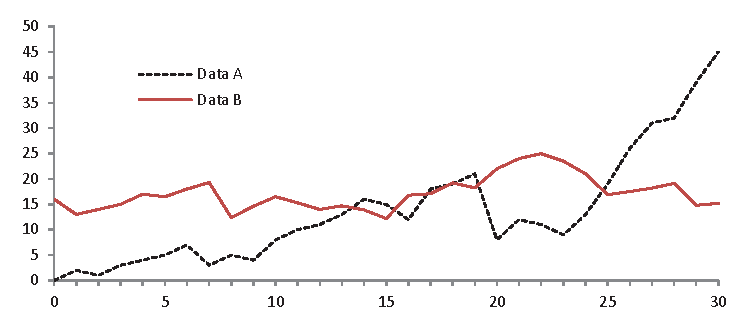
\includegraphics[width=\textwidth]{fig1.eps}
\caption{A figure caption is always placed below the illustration.
Please note that short captions are centered, while long ones are
justified by the macro package automatically.} \label{fig1}
\end{figure}

\begin{theorem}
This is a sample theorem. The run-in heading is set in bold, while
the following text appears in italics. Definitions, lemmas,
propositions, and corollaries are styled the same way.
\end{theorem}
%
% the environments 'definition', 'lemma', 'proposition', 'corollary',
% 'remark', and 'example' are defined in the LLNCS documentclass as well.
%
\begin{proof}
Proofs, examples, and remarks have the initial word in italics,
while the following text appears in normal font.
\end{proof}
For citations of references, we prefer the use of square brackets
and consecutive numbers. Citations using labels or the author/year
convention are also acceptable. The following bibliography provides
a sample reference list with entries for journal
articles~\cite{ref_article1}, an LNCS chapter~\cite{ref_lncs1}, a
book~\cite{ref_book1}, proceedings without editors~\cite{ref_proc1},
and a homepage~\cite{ref_url1}. Multiple citations are grouped
\cite{ref_article1,ref_lncs1,ref_book1},
\cite{ref_article1,ref_book1,ref_proc1,ref_url1}.

\subsubsection{Acknowledgements} Please place your acknowledgments at
the end of the paper, preceded by an unnumbered run-in heading (i.e.
3rd-level heading).

%
% ---- Bibliography ----
%
% BibTeX users should specify bibliography style 'splncs04'.
% References will then be sorted and formatted in the correct style.
%
% \bibliographystyle{splncs04}
% \bibliography{mybibliography}
%
\begin{thebibliography}{8}
\bibitem{ref_article1}
Author, F.: Article title. Journal \textbf{2}(5), 99--110 (2016)

\bibitem{ref_lncs1}
Author, F., Author, S.: Title of a proceedings paper. In: Editor,
F., Editor, S. (eds.) CONFERENCE 2016, LNCS, vol. 9999, pp. 1--13.
Springer, Heidelberg (2016). \doi{10.10007/1234567890}

\bibitem{ref_book1}
Author, F., Author, S., Author, T.: Book title. 2nd edn. Publisher,
Location (1999)

\bibitem{ref_proc1}
Author, A.-B.: Contribution title. In: 9th International Proceedings
on Proceedings, pp. 1--2. Publisher, Location (2010)

\bibitem{ref_url1}
LNCS Homepage, \url{http://www.springer.com/lncs}. Last accessed 4
Oct 2017
\end{thebibliography}
\end{document}
